\chapter{Calculating Quantum Corrected Free Energies Using a Single Step Perturbation Approach} \label{Chapter:single_step}

\section{Introduction}

The Introduction explained the importance of calculating accurate binding free energies for all systems using a relatively inexpensive method.  Also that to find a rigorous method that obeys the rules of statistical mechanics, total energies should be used.  This chapter provides the description and results of how this task was initially tackled.  Following a similar method described by Fox et al. \cite{fox_mm_to_qm} in that classical mechanics will be used to generate an ensemble of structures cheaply, then the Zwanzig equation \cite{zwanzig} will be used to perturb from this classical ensemble to a fully quantum one, making use of the extended thermodynamic cycle.  Fox et al. \cite{fox_mm_to_qm} briefly describe a few issues associated with this, the first being that due to the large size difference between the MM and QM total energies, the calculation of the exponential required for the Zwanzig equation (shown in equation \ref{eq:1_zwanzig}) is numerically unstable, however, numerical tricks can be used to calculate this \cite{Berg_maths}.  The second is that the number of classical snapshots required for convergence is too high.  This poses more of an issue, and it is because of this that we will apply the method to small test systems with considerably less configurational space available to sample that a larger system, e.g. a protein, to test convergence.


\section{Methods} \label{sec:results_ch1_methods}

\subsection{Classical Simulation Setup}

All classical simulations were performed in AMBER 10 \cite{amber_ref}, the initial structures for ethane and ethanol were generated using the MOE programme \cite{moe2009} parameterised using antechamber \cite{antechamber}.  TIP3P \cite{tip4p} was used as a solvent model and the generalised AMBER force field (GAFF) \cite{gaff} was used to describe ethane and ethanol.

%EQUILIBRATION

A fifteen step equilibration procedure was applied to two test systems, ethane in 133 TIP3P water and ethanol in 138 TIP3P water.  A small box size was selected to keep quantum simulations fast, as a caveat of this, only a 5 \AA{} nonbonded cutoff could be applied.  The equilibration procedure was as follows.  Initially the structure was minimised using 1000 steps of steepest descent and 1000 steps of conjugate gradient with a restraint of 1000 kcal/mol-\AA{}$^2$ on all non-hydrogen atoms.  This step was then repeated with the restraint removed on the oxygen atoms within the hydrogen.  After this the system was heated from 100 to 300K over 100ps, SHAKE \cite{shake} algorithm was used to allow for a 2fs time step.  This was performed in a canonical ensemble with a Langevin thermostat with a 3 ps$^{-1}$ collision constant with the same restraint as the previous step applied.  Then the volume was equilibrated by running within a isothermal-isobaric ensemble for 500ps.  The simulation was then cooled to 100K over 100ps.  Step one was repeated with the same restraint as the previous step.  This step was repeated a further eight times lowering the restraint each time to 500, 100, 50, 20, 10, 5, 2 kcal/mol-\AA{}$^2$ and removing it completely.  The system was then heated back up to 300K with no restraints present.


After the equilibration an MD simulation of 40 ns of ethane in 133 water was performed in the canonical ensemble and snapshots extracted at regular intervals.  For ethanol in water, a simulation length of 200 ns was run, the increase in length was to ensure the results were not being effected by correlated structures.

An additional test that will be described in more detail in the results section involved classical charge perturbations.  The starting point for these simulations was the equilibrated ethane in water system, and a simulation of 200 ns was run before extracting snapshots at regular intervals.

\subsection{Quantum Simulation Setup}

All quantum calculations were performed using ONETEP \cite{ONETEP} either using NGWFs or PAOs.  If NGWFs were used, the setup involved using NGWFs with radii of 8 bohr with 4 NGWFs describing heavy atoms and 1 for hydrogen.  When PAOs were used, a single zeta + polarisation basis set was used.

\subsection{Application of a Single Step Perturbation}

In order to perturb between two ensembles in a single step, the Zwanzig equation can be used.  This can be seen in equation \ref{eq:1_zwanzig}.

\begin{equation} \label{eq:1_zwanzig}
\ \Delta G = -k_B T  \ln \left\langle \exp \left[ - \frac{\Delta E_{QM-MM}}{k_BT} \right] \right\rangle_{MM}
\end{equation}


The large size difference between $E_{MM}$ and $E_{QM}$ makes the direct application of equation \ref{eq:1_zwanzig} numerically unstable.  As such, a method explained by Berg \cite{Berg_maths} can be used.  The method follows,

\begin{eqnarray}
\ C &=& A + B \\
\ \ln C &=& \ln (A+B) \\
\ &=& \ln \left[ max(A, B) \left( 1+ \frac{min(A, B)}{max(A, B)} \right)  \right] \\ \label{eq:berg}
\ &=& max(\ln A, \ln B)+ \ln(1+ \exp[min(\ln A, \ln B) - max ( \ln A, \ln B)]) .
\end{eqnarray}

Where A and B are,

\begin{equation}
\ \exp \left( - \frac{\Delta E_{QM-MM}}{k_BT}  \right) \\.
\end{equation}

The formula can then be used iteratively until all snapshots have been included.

\section{Results}

\subsection{Applying a Single Step Perturbation Approach to Non-Polar and Polar Test Systems} \label{sec:direct_application_of_single_step}

To validate the method simple test systems were selected, these included ethane in 133 water and ethanol in 138 water.  These were selected to show how the obtained results vary when applied to polar and non-polar systems.  Initially, the quantum calculations were performed with NGWFs as detailed in section \ref{sec:results_ch1_methods}.  In order to obtain classical structures a 40 ns MD simulation was performed, the resulting structures were divided into two groups, configurations that were generated in the first 20 ns (state A) and configurations generated in the second 20 ns (state B).  400 snapshots were then extracted from each state and the results compares in table \ref{table:ethane_NGWF}.

\begin{table}[ht]
 \caption{MM to QM perturbation applied to ethane using NGWFs, allowing upto 10\% of snapshots to be omitted due to SCF convergence errors.  All energies shown are in kcal/mol}
  \begin{center}
  \begin{tabular}{c|c|c|c}
   \hline\hline
 Number of snapshots & 1$^{st}$ 20.0 ns & 2$^{nd}$ 20.0 ns & Difference \\
 & $\Delta$ G & $\Delta$ G & $\Delta \Delta$ G  \\
\hline
400 & -1447906.57 & -1447912.01 & 5.44 \\
  \end{tabular}\label{table:ethane_NGWF}
 \end{center}
\end{table}
%
Examination of the structures that did not converge due to SCF convergence errors yielded no explanations.  The convergence issues came from the outer loop of ONETEP, the NGWF optimisation.

It is clear that 400 snapshots from state A and B are not enough to provide convergence of the method.  As such additional snapshots were calculated, but for speed, these snapshots were calculated using PAOs instead of NGWFs.  Simulation times for the single point energy calculations when using NGWFs were approximately 7 hours on 6 cores, whereas by using PAOs, this computational time lowered to 4 hours on 6 cores.  Additionally, by using PAOs the previous convergence issues were not present as only the density kernel is optimised.  By increasing the number of snapshots from each state to 1000 and applying this single step perturbation (SSP) method, $\Delta \Delta $G is still not 0.  These results can be seen in table \ref{table:ethane_PAO}.

\begin{table}[ht]
 \caption{MM to QM perturbation applied to ethane using PAOs.  All energies shown are in kcal/mol}
  \begin{center}
  \begin{tabular}{c|c|c|c}
   \hline\hline
 Number of snapshots & 1$^{st}$ 20.0 ns & 2$^{nd}$ 20.0 ns & Difference \\
 & $\Delta$ G & $\Delta$ G & $\Delta \Delta$ G  \\ [0.5ex]
\hline
1000 & -1442495.51 & -1442499.82 & 4.31 \\
  \end{tabular}\label{table:ethane_PAO}
 \end{center}
\end{table}

Investigating the lack of convergence present within the $\Delta \Delta$ G led to calculating the free energy as a function of the number of snapshots included.  In this way if the free energy is being dominated by one or a few snapshots it will become apparent.  The resulting graph can be seen in figure \ref{fig:ethane_PAO}.

\begin{center}
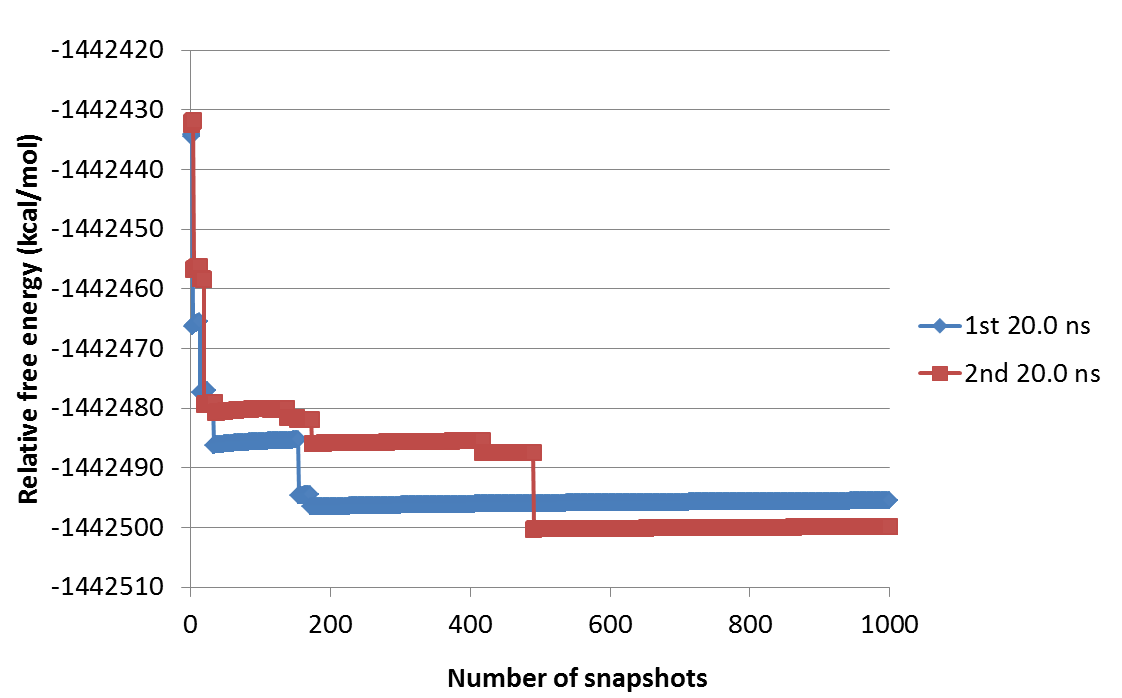
\includegraphics[width=15cm]{ethane_138_water_PAO.png}
 \captionof{figure}{Free energy as a function of the number of snapshots for ethane in 133 water, all values shown are in kcal/mol}\label{fig:ethane_PAO}
\end{center}

The ``sawtooth'' shape of the graph in figure \ref{fig:ethane_PAO} is characteristic of poor sampling \cite{good_practice_free_energy}.  In order to ensure that the lack of convergence in the $\Delta \Delta$ G was related to using a basis set with poor accuracy, when applying the SSP method to ethanol in 138 water, NGWFs were used.  Additionally the original MD simulation used to generate configurations was run for a longer time of 200ns to provide certainty of obtaining uncorrelated structures.  However, regardless of these additional measures taken to achieve convergence of $\Delta \Delta $ G, the difference is much larger (table \ref{table:ethanol_NGWF}) and 10\% of structures would not converge, an issue that, again, was not explained by further examination of these structures.

\begin{table}[ht]
 \caption{MM to QM perturbation applied to ethanol using NGWFs, allowing upto 10\% of snapshots to be omitted due to SCF convergence errors.  All energies shown are in kcal/mol}
  \begin{center}
  \begin{tabular}{c|c|c|c}
   \hline\hline
 Number of snapshots & 1$^{st}$ 20.0 ns & 2$^{nd}$ 20.0 ns & Difference \\
 & $\Delta$ G & $\Delta$ G & $\Delta \Delta$ G  \\ [0.5ex]
\hline
1000 & -1511726.64 & -1511765.45 & 38.81 \\
  \end{tabular}\label{table:ethanol_NGWF}
 \end{center}
\end{table}

\begin{center}
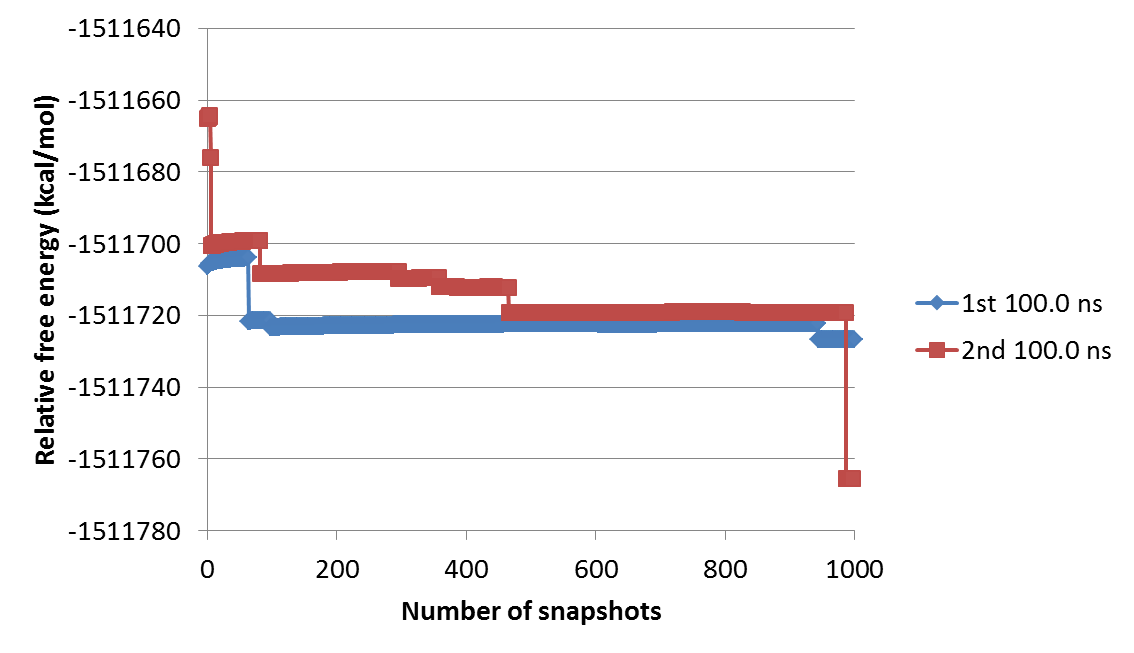
\includegraphics[width=15cm]{ethanol_138_water_NGWF.png}
 \captionof{figure}{Free energy as a function of the number of snapshots for ethanol in 138 water, all values shown are in kcal/mol}\label{fig:ethanol_NGWF}
\end{center}

Again plotting $\Delta \Delta$ G as a function of the number of snapshots, was then produced for ethanol in 138 water and shown in figure \ref{fig:ethanol_NGWF}.  This figure shows the catastrophic effect that one of these outlier structures can have on the free energy.  The largest effect to the free energy occurred within this 2nd 100 ns simulation of ethanol in 138 water.  The distributions of energies produced by the structures within this simulation were then compared.

Three energy distributions were produced from this simulation, these energies were the MM, QM and QM-MM distributions.  To analyse these distributions, they were plotted within box and whisker plots.  The ``box'' in the box and whisker plots shows the interquartile range (IQR) of the data, and the line in the middle of the box is the median.  This whisker length is 1.5 times the length of the IQR, any snapshots outside of this length can be thought of as an energetical outlier.

\begin{center}
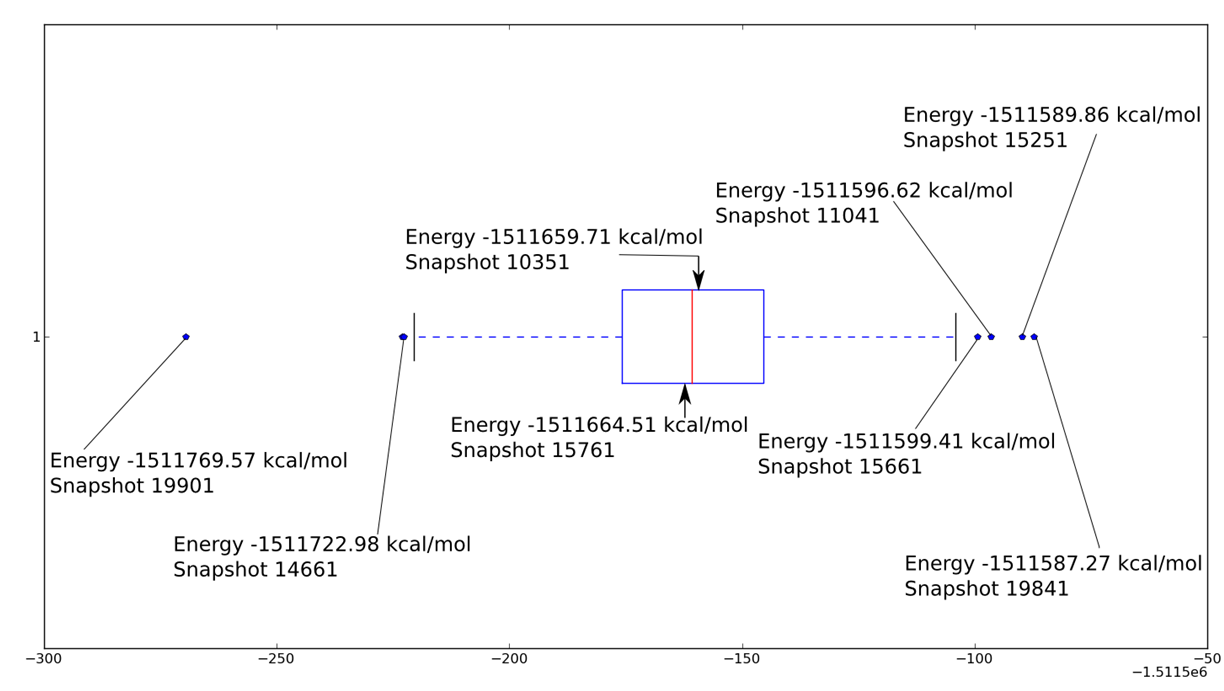
\includegraphics[width=15cm]{QM-MM_box_plot.png}
 \captionof{figure}{Energy difference distribution for the ethanol in 138 water, 2nd 200 ns, plotted in a box and whisker plot}\label{fig:QM-MM_box_plot}
\end{center}

Six outlier snapshots can be identified from figure \ref{fig:QM-MM_box_plot} and, for analysis purposes, two snapshots close to the median value were selected to show their location within the other distributions.  The box and whisker plot shows a large range of 182.30 kcal/mol within the energy differences.  Producing similar plots for the MM and QM energy distributions provides some interesting results.


\begin{center}
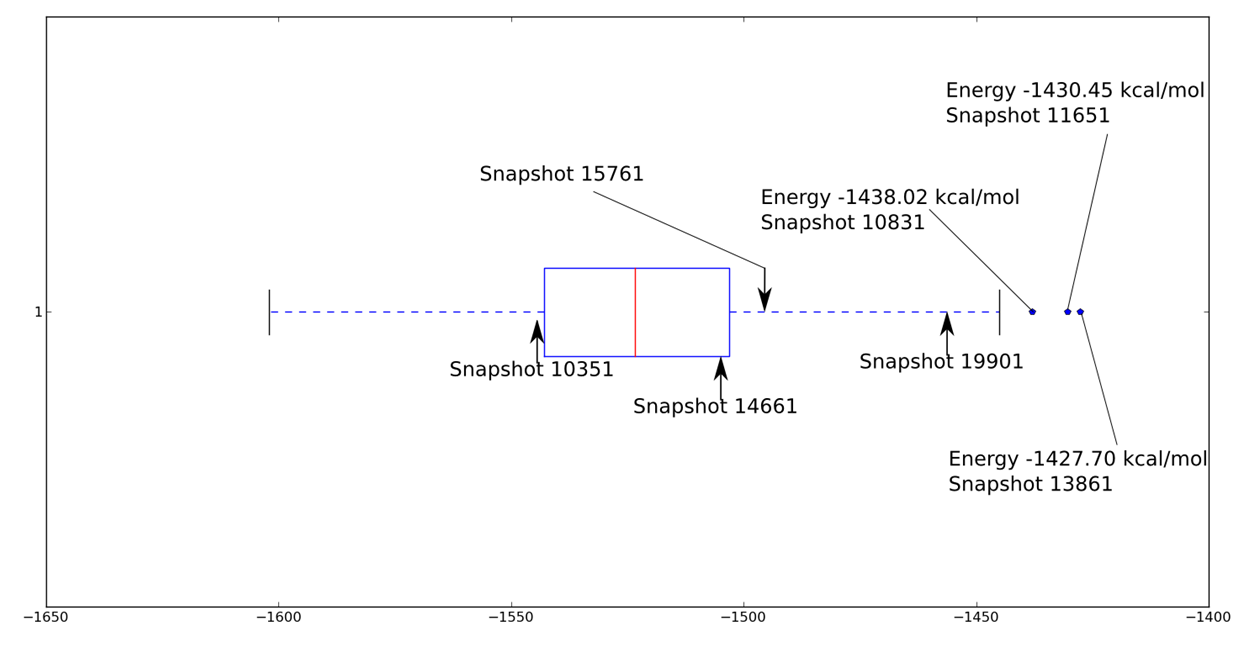
\includegraphics[width=15cm]{MM_box_plot.png}
 \captionof{figure}{MM energy distribution for the ethanol in 138 water, 2nd 200 ns, plotted in a box and whisker plot}\label{fig:MM_box_plot}
\end{center}

\begin{center}
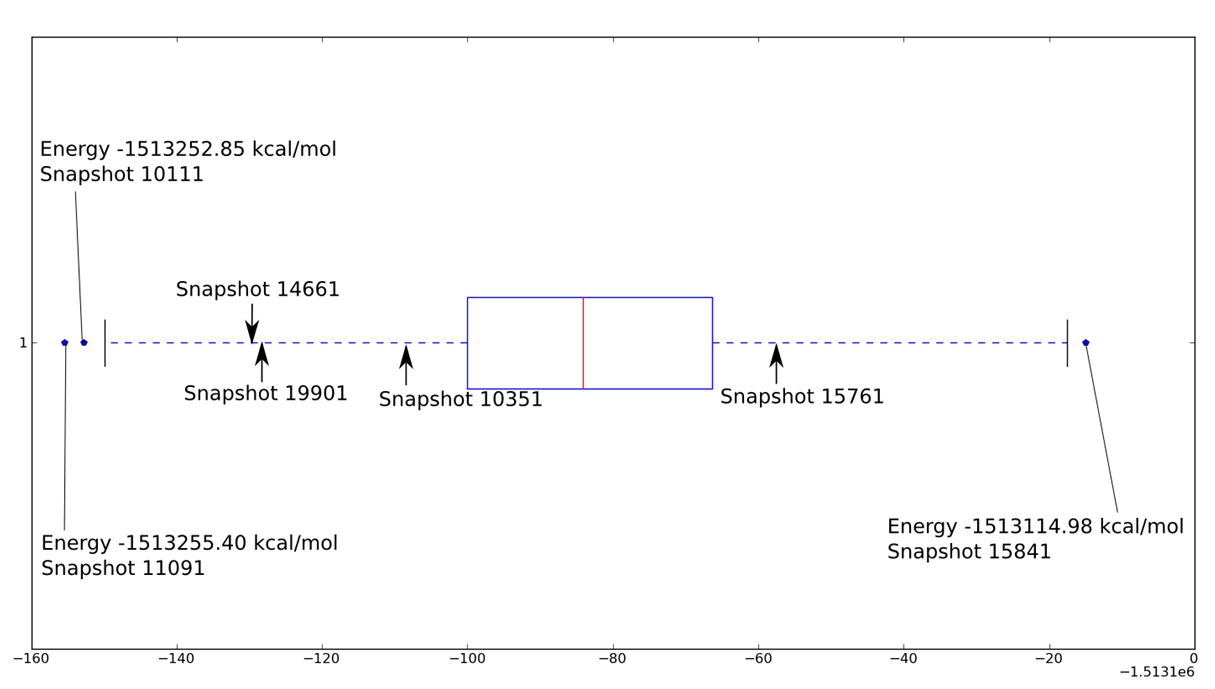
\includegraphics[width=15cm]{QM_box_plot.png}
 \captionof{figure}{QM energy distribution for the ethanol in 138 water, 2nd 200 ns, plotted in a box and whisker plot}\label{fig:QM_box_plot}
\end{center}

Comparing which snapshots were shown to be outlier snapshots in each distribution produced the following table (table \ref{table:outlier_snapshots}).

\begin{table}[ht]
 \caption{Outlier snapshots}
  \begin{center}
  \begin{tabular}{c|c|c}
   \hline\hline
 Energy Difference & QM & MM \\ [0.5ex]
\hline
19901 & 11901 & 10831 \\
14661 & 10111 & 11651 \\
15661 & 15841 & 13861 \\
11041 & & \\
15251 & & \\
19841 & & \\
  \end{tabular}\label{table:outlier_snapshots}
 \end{center}
\end{table}

Table \ref{table:outlier_snapshots} shows that for all three distribution, there are no common outliers.  Which proves that the large jumps present in figure \ref{table:ethanol_NGWF} attributed to the energy difference outliers are not present due to a structure being anomalous in either the MM or QM distributions.  Additionally, the examination of the positions of the snapshots identified as close to the median in the energy differences within the MM and QM distributions show that, in both cases, the snapshots are outside of the IQR.  However, because both of the snapshots appear on the same side of the MM and QM distributions i.e. either both snapshots appear on the more negative side of the IQR or both snapshots appear on the less negative side of the IQR, the snapshots appear close to the median in the energy difference distribution.  With regard to the outlier snapshots within the energy difference distribution, the more negative side of the distribution will have a larger effect on the free energy.  This is due to the calculation of the exponential of the negative energy present within the Zwanzig equation (equation \ref{eq:1_zwanzig}).  Finding these snapshots within the MM and QM distributions show them to be on different sides of the distributions.  This difference shows that the MM and QM configurational space does not overlap exactly, and this inexact overlap of configurational space causes these energy difference outliers.  

\subsection{Controlling the Level of Configurational Overlap to Measure the Convergence of the Free Energy}

In order to investigate the perturbation between different potentials, while controlling the degree of configurational space overlap, a test system was set up.  Calculating quantum energies are orders of magnitude more computationally expensive than classical energies, as such, the test system was between classical systems.  The test system of ethane in 133 water was used with the setup described within the methods section.  The MD simulation was then divided into two parts and 10000 snapshots were extracted at regular intervals and the charges present on ethane were then perturbed.  The standard charges on ethane used were obtained from antechamber \cite{antechamber}, these were -0.0941 on carbon and 0.0317 on hydrogen. The perturbations then involved changing these charges and calculating the new energies, these charges were changed by doubling them, tripling them etc.. up to eight times the charge.  The convergence of $\Delta \Delta$ G was then measured while lowering the configurational space overlap.


\begin{table}[ht]
 \caption{Calculating the free energy required to perturb the charges on ethane in 133 water from standard charges to increased charges.  Sampling performed using standard charges.  All energies shown are in kcal/mol}
  \begin{center}
  \begin{tabular}{c|c|c|c}
   \hline\hline
 Increased charge & 1$^{st}$ 100.0 ns & 2$^{nd}$ 100.0 ns & Difference \\
 & $\Delta$ G & $\Delta$ G & $\Delta \Delta$ G  \\
\hline
 Double & 2.800 & 2.798 & 0.002 \\
\hline
 Triple & 7.439 & 7.434 & 0.005 \\
\hline
 Quadruple & 13.898 & 13.886 & 0.012 \\
\hline
 Pentuple & 22.148 & 22.111 & 0.037 \\
\hline
 Sextuple & 32.231 & 32.108 & 0.123 \\
\hline
 Septuple & 43.957 & 43.635 & 0.322 \\
\hline
 Octuple & 57.365 & 56.751 & 1.206 \\
  \end{tabular}\label{table:charge_forward}
 \end{center}
\end{table}

Table \ref{table:charge_forward} shows that by lowering the amount of overlap present between the two states involved in the perturbation, the free energy does not converge.  The trend of $\Delta \Delta$ G is as expected, when perturbations are small the free energy converges.  Configurational space overlap is demonstrated in figure \ref{fig:bond_length} and \ref{fig:angles}.  Where, in figure \ref{fig:bond_length}, the carbon carbon bond length is measured when an MD simulation is performed using the altered charges.  Figure \ref{fig:angles} shows a similar analysis, but using the hydrogen-carbon-carbon angle of these MD simulations.  These figures show that as the charge is increased, both the bond length and angle is increased slightly.  


\begin{center}
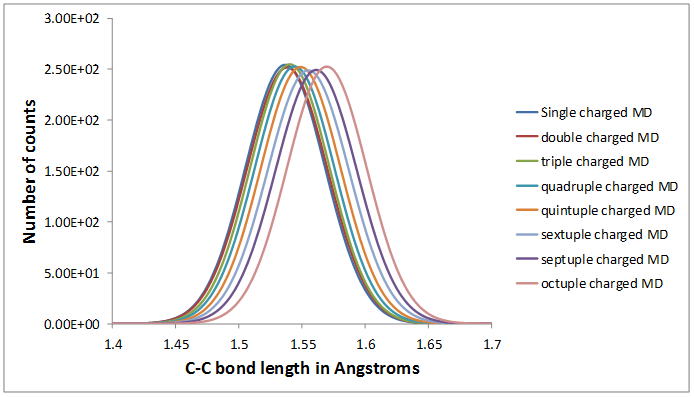
\includegraphics[width=15cm]{bond_lengths_charge.png}
 \captionof{figure}{Carbon-carbon bond length within 8 different MD simulations with different partial charges on ethane}\label{fig:bond_length}
\end{center}

\begin{center}
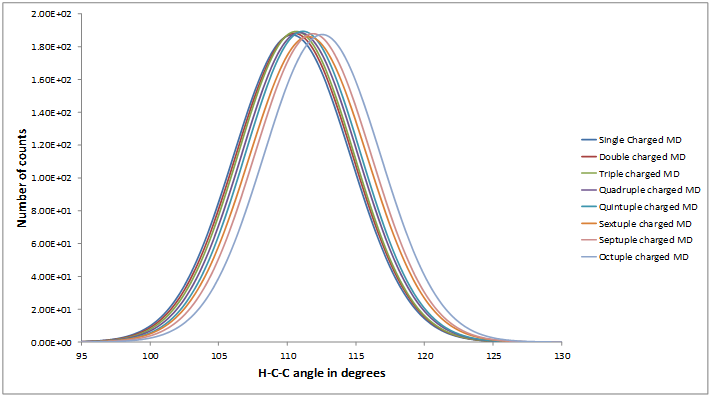
\includegraphics[width=15cm]{angles_charge.png}
 \captionof{figure}{Carbon-carbon-hydrogen angle within 8 different MD simulations with different partial charges on ethane}\label{fig:angles}
\end{center}

Noticing how poor the configurational space overlap is between the standard and octuple charged systems, the reverse calculation was performed.  This involved running an MD simulation at the desired charge and perturbing to a standard charged system.  Free energy is a state function, so the reverse process should be the negative of the forward process.

\begin{table}[ht]
 \caption{Calculating the free energy required to perturb the charges on ethane in 133 water, from standard charges to an increased charge.  Sampling performed using the increased charges.  All energies shown are in kcal/mol}
  \begin{center}
  \begin{tabular}{c|c|c|c}
   \hline\hline
 Increased charge & 1$^{st}$ 100.0 ns & 2$^{nd}$ 100.0 ns & Difference \\
 & $\Delta$ G & $\Delta$ G & $\Delta \Delta$ G  \\
\hline
 Double & 2.773 & 2.771 & 0.002 \\
\hline
 Triple & 7.290 & 7.293 & -0.003 \\
\hline
 Quadruple & 13.386 & 13.428 & -0.042 \\
\hline
 Pentuple & 20.864 & 20.795 & 0.069 \\
\hline
 Sextuple & 29.422 & 29.228 & 0.194 \\
\hline
 Septuple & 36.360 & 37.766 & -1.406 \\
\hline
 Octuple & 43.939 & 45.746 & -1.807 \\
  \end{tabular}\label{table:charge_reverse}
 \end{center}
\end{table}

\begin{table}[ht]
 \caption{The difference between perturbations, each value is the average of the 1$^{st}$ and 2$^{nd}$ 100ns.  All energies shown are in kcal/mol}
  \begin{center}
  \begin{tabular}{c|c|c|c}
   \hline\hline
 Increased charge & standard to increased charge & increased charge to standard & Difference \\
 & $\Delta$ G & $\Delta$ G & $\Delta \Delta$ G  \\
\hline
 Double & 2.799 & 2.772 & 0.027 \\
\hline
 Triple & 7.437 & 7.292 & 0.145 \\
\hline
 Quadruple & 13.892 & 13.407 & 0.485 \\
\hline
 Pentuple & 22.130 & 20.830 & 1.300 \\
\hline
 Sextuple & 32.170 & 29.325 & 2.845 \\
\hline
 Septuple & 43.796 & 37.063 & 6.733 \\
\hline
 Octuple & 57.058 & 44.843 & 12.215 \\
  \end{tabular}\label{table:charge_differences}
 \end{center}
\end{table}


The results show poor convergence of the free energy.  This shows that when the configurational space does not overlap exactly the forward and reverse process does not converge.  The lack of overlap here is small, but the overlap between classical and quantum configurational space has been shown to be poor.  This offers some explanation toward the poor convergence of the MM to QM.  It is clear that without sampling a large amount of configurational space, the free energy from MM to QM will not converge.  Also the cost of running quantum calculations on 1000 snapshots for ethane in 133 water is a manageable computational cost, but for a larger, more biologically relevant system, 1000 snapshots will be extremely computationally expensive.  So several post-processing methods were applied to try and converge these free energies and the results are shown in the next section.

\subsection{Methods to Converge the Free Energy}

The largest effect an energy difference outlier had on the convergence of free energies was observed for ethanol in 138 water in the 2$^{nd}$ 100 ns.  Because of this, all attempts to converge the free energy, using the data already obtained, will be for this system.  Section \ref{sec:direct_application_of_single_step} shows that it is impossible to predict where energy difference outliers will occur by examining only the classical or quantum energies.  Because of this, the first attempt to better converge the free energy was to subtract the average energy from both energy distibutions,

\begin{equation}
\ \Delta E = (E_{i}^{MM}- \langle E^{MM}\rangle) - (E_{i}^{QM}-\langle E^{QM}\rangle) \\.
\end{equation}
%
Where the subscript $i$ represents the $i^{th}$ structure, $\langle E_{i}^{MM}\rangle$ is the average classical energy.

The results, shown in table \ref{table:ethanol_relative_energies_NGWF}, display the same poor convergence of table \ref{table:ethanol_NGWF}.  Applying the Zwanzig equation \cite{zwanzig} as a function of the number of snapshots, provides large ``jumps'' in free energy again (figure \ref{fig:ethanol_relative_energies_NGWF}), showing that subtracting the average from each energy distribution cannot converge the free energy.

\begin{table}[ht]
 \caption{MM to QM perturbation applied to ethanol using NGWFs, each energy distribution has the average energy subtracted from it.  Allowing upto 10\% of snapshots to be omitted due to SCF convergence errors.  All energies shown are in kcal/mol}
  \begin{center}
  \begin{tabular}{c|c|c|c}
   \hline\hline
 Number of snapshots & 1$^{st}$ 20.0 ns & 2$^{nd}$ 20.0 ns & Difference \\
 & $\Delta$ G & $\Delta$ G & $\Delta \Delta$ G  \\
\hline
1000 & -66.04 & -104.51 & 38.47 \\
  \end{tabular}\label{table:ethanol_relative_energies_NGWF}
 \end{center}
\end{table}


\begin{center}
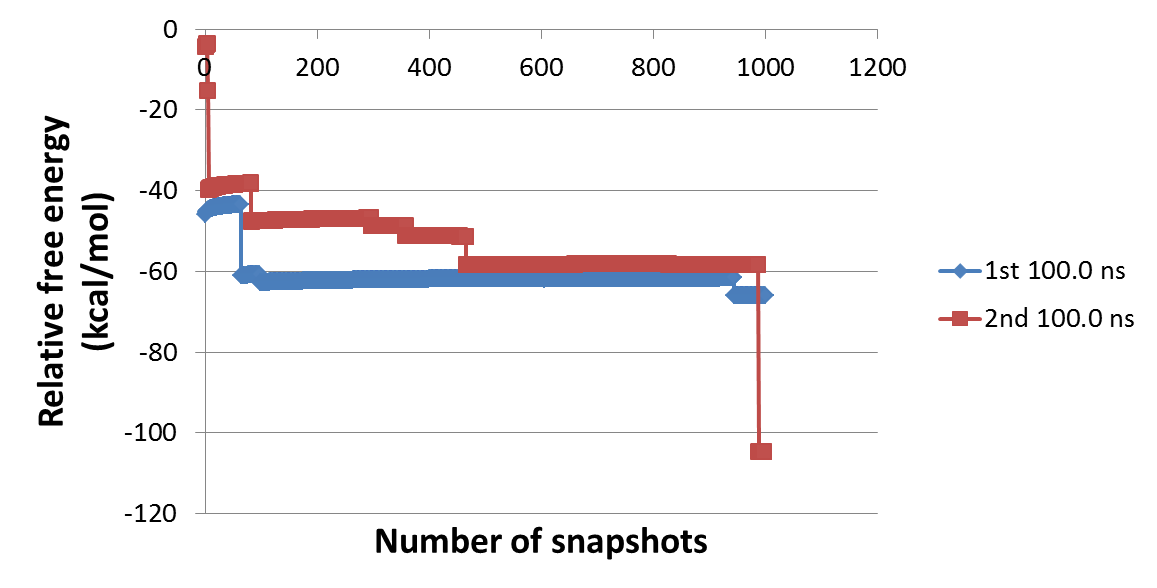
\includegraphics[width=15cm]{ethanol_138_water_NGWF_relative_energy.png}
 \captionof{figure}{Free energy as a function of the number of snapshots included for ethanol in 138 water, subtracting the average energy from energy distributions}\label{fig:ethanol_relative_energies_NGWF}
\end{center}

Following this, the distribution of the energy differences was examined and  found to be Gaussian.  The combination of the energy differences for the 1$^{st}$ and 2$^{nd}$ 100ns is shown in figure \ref{fig:energy_difference_gaussian}.  Although the distribution fits a Gaussian well, the energy differences show a large range: approximately 138 kcal/mol.  When considering that it is the exponential of these energy differences that are calculated, 138 is extremely large.  Nevertheless, by introducing a Gaussian to act as a smoothing function, the low-energy tail may be better described and provide convergence of the free energy.

\begin{center}
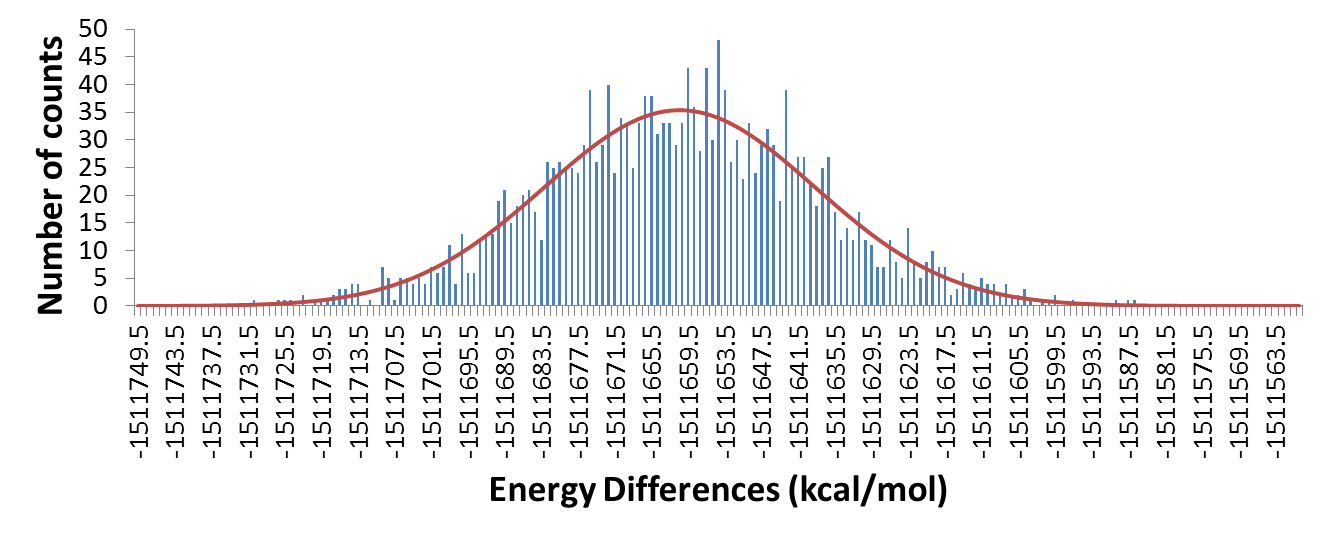
\includegraphics[width=15cm]{energy_difference_gaussian.png}
 \captionof{figure}{Energy differences for the full 200 ns of data for ethanol in 138 water}\label{fig:energy_difference_gaussian}
\end{center}


Using a Gaussian distribution to describe the energy differences for both the 1$^{st}$ and 2$^{nd}$ 100ns separately, then applying equation \ref{eq:gaussian_free_energy}, the free energy can be found.  By using these Gaussian distributions, we approximate how the distribution would look if we could sample infinitely.  To do this, the Gaussian is used as the probability density for $\Delta E$, then the following can be used\cite{good_practice_free_energy},

\begin{eqnarray}
\ \Delta G &=& -k_BT \ln \int P(\Delta E) \exp \left[ - \frac{\Delta E}{k_BT} \right] dE \nonumber \\ \label{eq:gaussian_free_energy}
\ &=& -k_BT \left\langle - \frac{\Delta E}{k_BT} \right\rangle .
\end{eqnarray}
%
Where $P(\Delta E)$ is the probability density of $\Delta E$, $k_B$ is the Boltzmann constant and $T$ is the temperature.

In practice, however, the distribution was divided into small segments and the following equation was used along with the trapezoid rule for integration,

\begin{equation} \label{eq:gaussian_free_energy_segments}
\ \Delta G = -k_B T\ln \sum^{n_{Bars}}_{i=1}P(\Delta E_i) \exp \left[ -\frac{\Delta E_i}{k_BT} \right] \\.
\end{equation}

In order to calculate the required exponential of the energy difference for equation \ref{eq:gaussian_free_energy_segments}, Berg's \cite{Berg_maths} formula for the calculation of large exponentials (equation \ref{eq:berg}) must be used, as before in section \ref{sec:direct_application_of_single_step}.  In this case, however, by using the rules for dealing with logarithms, $\ln A$ will be the following,

\begin{equation}
\ \ln A= \ln (P(\Delta E_i))-\frac{\Delta E_i}{k_BT} \\.
\end{equation}

When using bin widths of 1 kcal/mol, where ``bin'' in this case refers to the small segments the Gaussian distribution is divided into, the results can be seen in table \ref{table:ethanol_using_gaussian}.

\begin{table}[ht]
 \caption{Using Gaussian distributions for the 1$^{st}$ and 2$^{nd}$ 100 ns, then integrating over the probability distribution}
  \begin{center}
  \begin{tabular}{c|c|c|c}
   \hline\hline
 1000 snapshots & 1$^{st}$ 100.0 ns & 2$^{nd}$ 100.0 ns & Difference \\
 Bin width (kcal/mol) & $\Delta$ G & $\Delta$ G & $\Delta \Delta$ G  \\
\hline
1 & -1512064.46 & -1512070.75 & 6.29 \\
  \end{tabular}\label{table:ethanol_using_gaussian}
 \end{center}
\end{table}

Although the free energy is still not converged, the difference is a great deal smaller, down to 6.29 kcal/mol.  This is a promising result, and the application of smoothing functions will be further investigated.  For comparison, this method was applied directly to the histogram that was used to generate the Gaussians.  The histograms were initially normalised so that the area underneath them was equal to 1, equation \ref{eq:berg} was then applied using this new count.  The results are shown in table \ref{table:ethanol_using_histogram}.

\begin{table}[ht]
 \caption{Using the histograms for the 1$^{st}$ and 2$^{nd}$ 100 ns}
  \begin{center}
  \begin{tabular}{c|c|c|c}
   \hline\hline
 1000 snapshots & 1$^{st}$ 100.0 ns & 2$^{nd}$ 100.0 ns & Difference \\
 Bin width (kcal/mol) & $\Delta$ G & $\Delta$ G & $\Delta \Delta$ G  \\
\hline
10 & -1511729.23 & -1511759.23 & 30.00 \\
\hline
1 & -1511723.55 & -1511762.55 & 39.00 \\
\hline
0.1 & -1511722.84 & -1511761.63 & 38.79 \\
  \end{tabular}\label{table:ethanol_using_histogram}
 \end{center}
\end{table}

As expected without a smoothing function, the free energy does not converge.  The funtional form of the Gaussian used as the smoothing function was the following,

\begin{equation}
\ P(\Delta E)=N \exp \left[ - \alpha ( E- E_0)^2  \right] \\.
\end{equation}

By integration of the following equation (equation \ref{eq:analytical_free_energy}) the analytical solution to the free energy can be obtained.  

\begin{eqnarray}
\ \Delta G &=& -k_BT \ln \left\langle \exp \left[-\frac{\Delta E}{k_BT}\right] \right\rangle \\
&=& -k_{B}T \ln \frac{\int P(\Delta E) \exp \left[ \frac{-\Delta E}{k_BT}\right] d \Delta E}{\int P(\Delta E)d \Delta E} \label{eq:analytical_free_energy} \\
\ &=& -k_B T \ln \frac{I_1}{I_2}
\end{eqnarray}

$I_2$ is the simpler of the two integrals, as such it will be solved first.

\begin{equation} \label{eq:I2}
\ I_2 =\int_{-\infty}^{\infty} \exp \left[ - \alpha (\Delta E- \Delta E_0)^2  \right] dE \\.
\end{equation}

Setting $y=\sqrt{\alpha}(\Delta E- \Delta E_0)$,

\begin{eqnarray}
\ y &=& \sqrt{\alpha}\Delta E-\sqrt{\alpha} \Delta E_0 \\
\ \frac{dy}{d\Delta E} &=& \sqrt{\alpha} \\
\ d\Delta E &=& \frac{1}{\sqrt{\alpha}}dy \label{eq:dE} .
\end{eqnarray}
%
Substituting equation \ref{eq:dE} into equation \ref{eq:I2} and using the rule of integrating Gaussians, $\int_{-\infty}^{\infty} \exp [ -x^2] dx= \sqrt{\pi}$, leads to,

\begin{equation}
\ I_2 = \frac{1}{\sqrt{\alpha}}\int_{-\infty}^{\infty} \exp [-y^2] dy = \sqrt{\frac{\pi}{\alpha}} \\.
\end{equation}
%
Now, examining the numerator of equation \ref{eq:analytical_free_energy},

\begin{eqnarray}
\ I_1 &=& \int_{-\infty}^{\infty} \exp\left[ -\beta \Delta E \right] \exp \left[ - \alpha(\Delta E- \Delta E_0)^2 \right] d \Delta E \\
\ &=& \int_{-\infty}^{\infty} \exp\left[ -\beta \Delta E- \alpha(\Delta E- \Delta E_0)^2 \right] d \Delta E
\end{eqnarray}
%
Then, working on the exponent,

\begin{eqnarray}
\ & & -\beta \Delta E- \alpha(\Delta E- \Delta E_0)^2 \\
\ &=& - \left[ \beta \Delta E + \alpha  \Delta E^2 + \alpha \Delta E^2_0 - 2 \alpha\Delta E\Delta E_0 \right] \\
\ &=& - \left[\Delta E \left( \beta -  2\alpha\Delta E_0 \right) + \alpha \Delta E^2 + \alpha \Delta E^2_0 \right] \\
\ &=& - \alpha \left[ \Delta E \left( \frac{\beta}{\alpha} -  2 \Delta E_0 \right)+ \Delta E^2 +  \Delta E^2_0  \right] \\
\ &=& - \alpha [ \Delta E^2 + 2\Delta E \left( \frac{\beta}{2\alpha} -  \Delta E_0 \right)+ \left( \frac{\beta}{2\alpha} -  \Delta E_0 \right)^2 + \Delta E^2_0 \nonumber \\
& & - \left( \frac{\beta}{2\alpha} - \Delta E_0 \right)^2 ] \\
&=& - \alpha \left[ \left( \Delta E + \left(\frac{\beta}{2\alpha}- \Delta E_0 \right) \right)^2 + \Delta E_0 - \left( \frac{\beta}{2 \alpha}- \Delta E_0 \right)^2  \right] \\
\ &=& - \alpha \left[ \left( \Delta E + \left(\frac{\beta}{2\alpha}- \Delta E_0 \right) \right)^2 - \frac{\beta^2}{4\alpha^2} + \frac{\beta \Delta E_0}{\alpha} \right] \\
\ &=& - \alpha \left( \Delta E + \left(\frac{\beta}{2\alpha}- \Delta E_0 \right) \right)^2 - \frac{\beta^2}{4\alpha} + \beta \Delta E_0 .
\end{eqnarray}
%
Therefore,

\begin{eqnarray}
\ I_1 &=& \int_{-\infty}^{\infty} \exp \left[ - \alpha (\Delta E-\Delta E_0)^2 - \beta \Delta E  \right] d \Delta E \\
\ &=& \int_{-\infty}^{\infty} \exp \left[ -\alpha \left(\Delta E + \left(\frac{\beta}{2\alpha}- \Delta E_0 \right) \right)^2 - \frac{\beta^2}{4\alpha} + \beta \Delta E_0 \right] d \Delta E \\
\ &=& \exp \left[ - \frac{\beta^2}{4\alpha} + \beta \Delta E_0 \right] \int_{\infty}^{\infty} \exp \left[ - \alpha \left( \Delta E + \left( \frac{\beta}{2\alpha}- \Delta E_0\right)\right)^2 \right] d \Delta E .
\end{eqnarray}
%
Then,

\begin{eqnarray}
\ x &=& \sqrt{\alpha}\left[ \Delta E+\left( \frac{\beta}{2 \alpha}- \Delta E_0 \right)\right] \\
\ \frac{dx}{d\Delta E} &=& \sqrt{\alpha} \\
\ d\Delta E &=& \frac{1}{\sqrt{\alpha}} dx .
\end{eqnarray}
%
$I_1$ is then,

\begin{eqnarray}
\ I_1 &=& \frac{1}{\sqrt{\alpha}}\exp \left[-\frac{\beta^2}{4\alpha}+ \beta \Delta E_0 \right] \int_{-\infty}^{\infty} \exp \left[ - x^2 \right] dx \\
\ &=& \sqrt{\frac{\pi}{\alpha}}\exp \left[-\frac{\beta^2}{4\alpha}+ \beta \Delta E_0 \right] .
\end{eqnarray}
%
Combining $I_1$ and $I_2$ gives,

\begin{eqnarray}
\ \frac{I_1}{I_2} &=& \left\langle \exp \left[ - \beta \Delta E \right] \right\rangle \\
&=& \exp \left[ - \frac{\beta^2}{4\alpha}+ \beta \Delta E_0 \right] .
\end{eqnarray}
%
Inserting this back into the Zwanzig equation,

\begin{eqnarray}
\ \Delta G &=& - \beta^{-1} \ln \left\langle \exp \left[ - \beta \Delta E \right] \right\rangle \\
\ &=& - \beta ^{-1} \ln \frac{I_1}{I_2} \\
\ &=& - \beta^{-1} \ln \left( \exp \left[ - \frac{\beta^2}{4\alpha}+ \beta \Delta E_0 \right] \right) \\
\ &=& - \beta^{-1} \left( \frac{\beta^2}{4\alpha}- \beta \Delta E_0  \right) \\ \label{eq:gaussian_free_energy_analytical}
\ &=& \Delta E_0 - \frac{\beta}{4 \alpha}
\end{eqnarray}

The free energy can then be calculated directly from the exponents used from the Gaussian used to fit the distribution.

The exponents fitted when using the full histogram are shown in table \ref{table:gaussian_exponents} and the free energies calculated when using these exponents within equation \ref{eq:gaussian_free_energy_analytical} are shown in table \ref{table:gaussian_exponents_free_energy}.  Along with these free energies, are the resulting free energies when the sample size for the histogram is reduced and the Gaussian re-fitted.  When lowering the sample size, the snapshots selected were spread evenly throughout the simulation.

\begin{table}[ht]
 \caption{Exponents used for the Gaussian distributions when using the full histograms for the 1$^{st}$ and 2$^{nd}$ 100 ns}
  \begin{center}
  \begin{tabular}{c|c|c|c}
   \hline\hline
 coefficient & 1$^{st}$ 100.0 ns & 2$^{nd}$ 100.0 ns & Difference \\
\hline
$\alpha$ & 0.0010276 & 0.0010126 & 0.000015 \\
\hline
E$_0$ & -1511661.01 & -1511660.96 & -0.06 \\
  \end{tabular}\label{table:gaussian_exponents}
 \end{center}
\end{table}

\begin{table}[ht]
 \caption{ Free energies obtained when using a Gaussian probability density along with equation \ref{eq:gaussian_free_energy_analytical} for the 1$^{st}$ and 2$^{nd}$ 100 ns}
  \begin{center}
  \begin{tabular}{c|c|c|c}
   \hline\hline
 & 1$^{st}$ 100.0 ns & 2$^{nd}$ 100.0 ns & Difference \\
 & $\Delta$ G (kcal/mol) & $\Delta$ G (kcal/mol) & $\Delta \Delta$ G (kcal/mol) \\
\hline
1000 & -1512069.09 & -1512075.07 & 5.98 \\
 \hline
500 & -1512087.09 &-1512076.93 & -10.16 \\
 \hline
100 & -1512232.73 & -1512010.76 & -221.97 \\
  \end{tabular}\label{table:gaussian_exponents_free_energy}
 \end{center}
\end{table}

\begin{center}
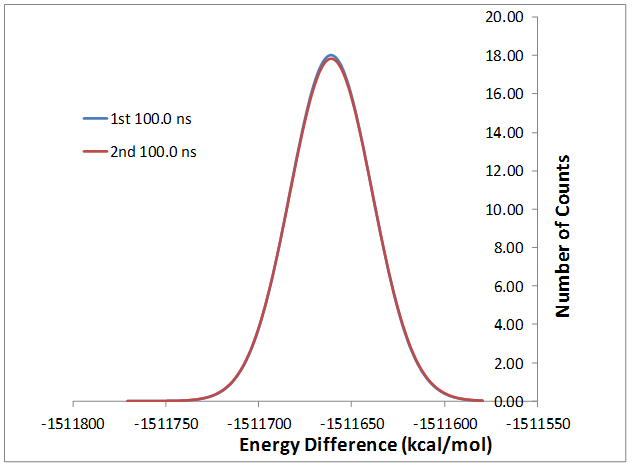
\includegraphics[width=10cm]{overlapping_gaussians.png}
 \captionof{figure}{The Gaussian distributions for the 1$^{st}$ and 2$^{nd}$ 100 ns}\label{fig:overlapping gaussians}
\end{center}


The difference in free energies is surprising when considering the small difference between the exponents of the Gaussian distribution.  Figure \ref{fig:overlapping gaussians} shows the two distributions overlapping to give an indication of how similar these distributions are.  These results led to a simple numerical test to find how sensitive these exponents are.  First, $\Delta \Delta$ G can be calculated by,

\begin{eqnarray}
\ \Delta \Delta G &=& \left( E_0^{(1)} - \frac{1}{4 \alpha_1 k_B T} \right) - \left( E_0^{(2)} -  \frac{1}{4 \alpha_2 k_B T} \right) \\
\ &=& \Delta E_0 - \frac{1}{4 \alpha_1 k_B T} + \frac{1}{4 \alpha_2 k_B T} \\
\ &=& \Delta E_0 -  \frac{1}{\alpha_1} + \frac{1}{\alpha_2} .
\end{eqnarray}
%
By setting $\Delta E_0$ to 0, the $\alpha$ exponents can be tested.  The aforementioned numerical test then involved setting $\alpha_1$ to values ranging from 0.001 to 0.999 in incremental steps of 0.001 and $\alpha_2$ was calculated to be $\alpha_1 +1 \%$ and $\alpha_1 -1 \%$.  The two $\Delta \Delta G$ values obtained were then compared and are shown in figure \ref{fig:alpha_exponent_sensitivity}.

\begin{center}
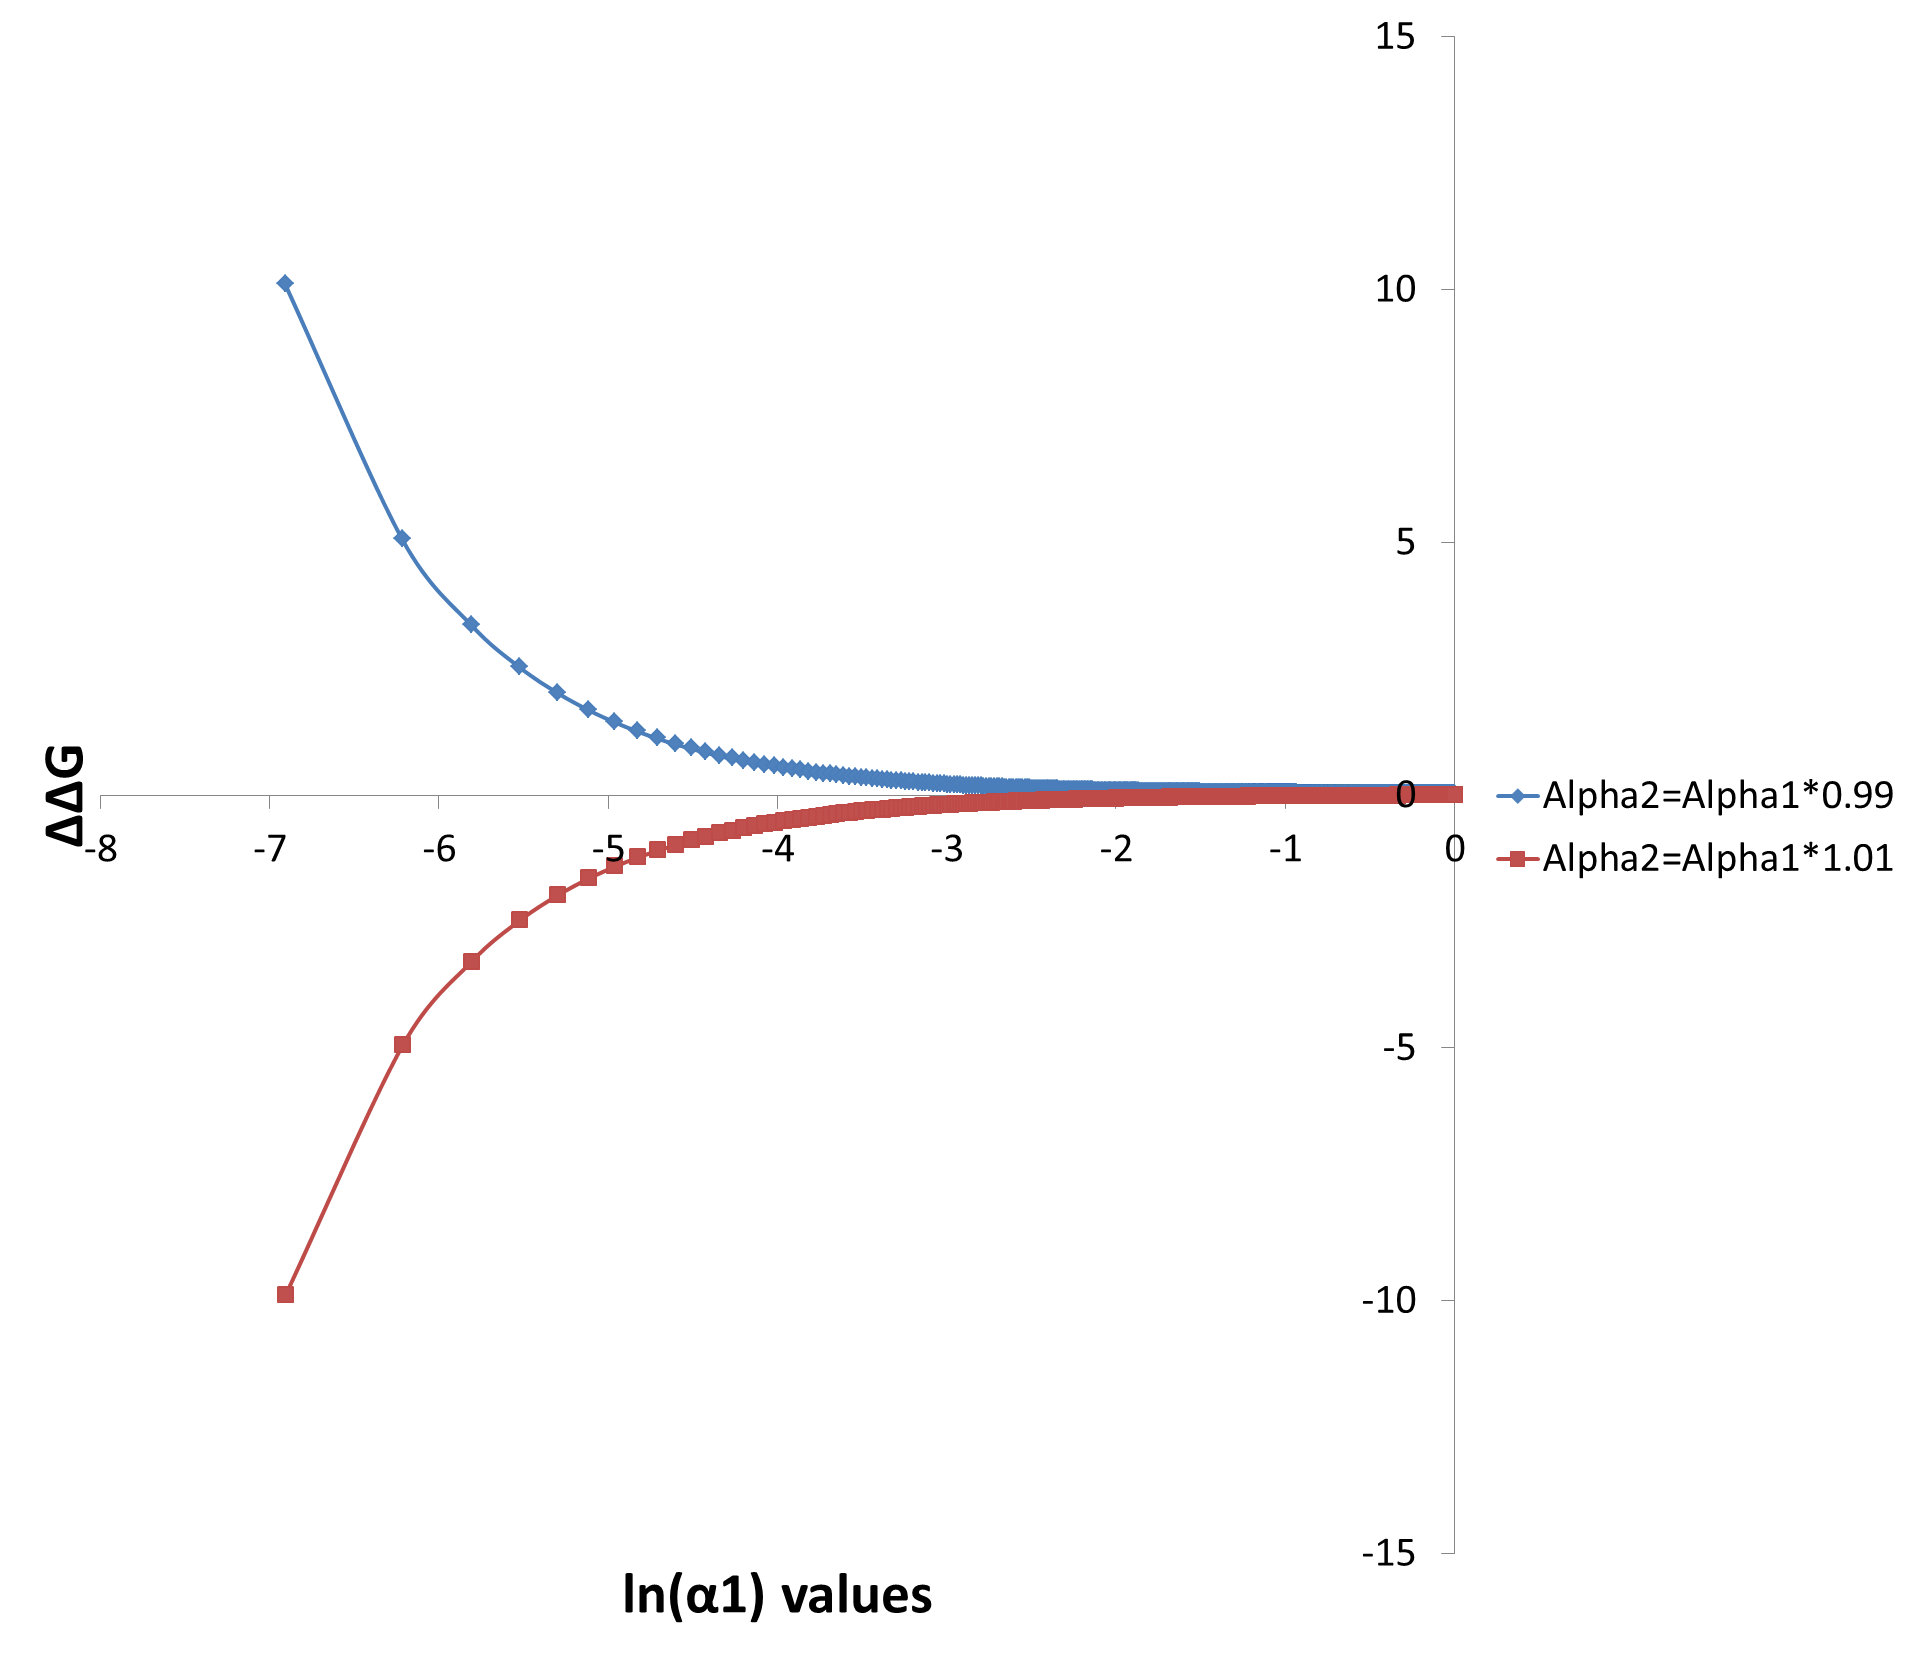
\includegraphics[width=15cm]{alpha_exponent_sensitivity.png}
 \captionof{figure}{The sensitivity of the $\alpha$ exponents used in equation \ref{eq:gaussian_free_energy_analytical} }\label{fig:alpha_exponent_sensitivity}
\end{center}


It is clear that when $\alpha$ is very small there is little room for any error.  However, the relative free energy for the system in table \ref{table:gaussian_exponents_free_energy} shows a reduction from applying the Zwanzig equation directly.  The reason for this can be found when considering that the exponential average is not calculated, so the low-energy tail of the distribution is not given unfair weighting.  To avoid this exponential averaging issue, the cumulant expansion of the free energy was considered\cite{cumulant_expansion_cutoff}.  This is simply the expansion of the Zwanzig equation (equation \ref{eq:gaussian_free_energy}) in a Taylor series \cite{Stat_mech}, the derivation follows.


Firstly we must specify the functional form that will be used,

\begin{eqnarray}
\ \Delta G &=& - \frac{1}{\beta} \ln \left\langle \exp \left[ - \beta \Delta E \right] \right\rangle \\ \label{eq:cumulant_step2}
\ &=& - \frac{1}{\beta} \ln \left\langle \sum^{\infty}_{l=0} \frac{(-\beta \Delta E)^l}{l!} \right\rangle \\ \label{eq:cumulant_step3}
\ &=& - \frac{1}{\beta} \ln \left( 1+ \sum^{\infty}_{l=1} \frac{(-\beta)^l}{l!} \left\langle \Delta E^l \right\rangle_0 \right) .
\end{eqnarray}

The step from equation \ref{eq:cumulant_step2} to \ref{eq:cumulant_step3} is performed as $\ln(1+x)$ can be expanded in a Maclaurin series (expansion of a function using a Taylor series at 0).

\begin{eqnarray}
\ f(x) &=& \sum_{n=0}^{\infty} f^{(n)}(a) \frac{(x-a)^n}{n!} \\
\ f(a) &=& \ln (1+a) \nonumber \\
\ f^{\prime} (a) &=& (1+a)^{-1} \nonumber \\
\ f^{\prime\prime} (a) &=& -(1+a)^{-2} \nonumber \\
\ f^{\prime\prime\prime} (a) &=& 2(1+a)^{-3} \nonumber \\
\ f^{\prime\prime\prime\prime} (a) &=& -6(1+a)^{-4} \nonumber \\
\ & & \cdots \nonumber \\
\ a &=& 0 \nonumber \\
\ f(x) &=& \ln (1+0) + (1+0)^{-1} \frac{x}{1!} + -(1+0)^{-2} \frac{x^2}{2!}+2(1+0)^{-3}\frac{x^3}{3!} \nonumber \\
& & - 6(1+0)^{-4} \frac{x^4}{4!} \\
\ &=& 0 + x - \frac{x^2}{2} + \frac{2x^3}{6} - \frac{6x^4}{24} \\
\ &=& 0 + x - \frac{x^2}{2} + \frac{x^3}{3} + \frac{x^4}{4} \\
\ &=& \sum_{k=1}^{\infty} (-1)^{n-1} \frac{x^n}{n} \label{eq:logarithm_expansion}
\end{eqnarray}

Combining equation \ref{eq:cumulant_step3} and \ref{eq:logarithm_expansion},

\begin{equation} \label{eq:cumulant_free_energy}
\ \Delta G = - \frac{1}{\beta} \sum_{k=1}^{\infty} (-1)^{k-1} \frac{1}{k} \left( \sum_{l=1}^{\infty} \frac{(-\beta)^l}{l!} \left\langle \Delta E_1^l \right\rangle \right)
\end{equation}

Equating \ref{eq:cumulant_free_energy} to the cumulant generating function, equation \ref{eq:cumulant_generating_function}, and cancelling a factor of $1/\beta$,

\begin{equation} \label{eq:cumulant_generating_function}
\ \Delta G = \sum_{k=1}^{\infty} \frac{(-\beta)^{k-1}}{k!} \omega_k \\.
\end{equation}

Extracting powers of $\beta^1$

\begin{eqnarray}
\ -\beta \omega_1 &=& - \beta \langle \Delta E \rangle_0 \nonumber \\
\ \omega_1 &=& \langle \Delta E \rangle_0 .
\end{eqnarray}

Next, extracting powers of $(\beta)^2$,

\begin{eqnarray}
\ \frac{(-\beta)^2}{2} \omega_2 &=& \left( \frac{(-\beta^2)}{2} \langle \Delta E^2 \rangle_0 \right) - \frac{1}{2}\left( \frac{(-\beta)}{1} \langle \Delta E \rangle_0 \right)^2 \\
\ &=& \frac{(-\beta)^2}{2}\langle \Delta E^2 \rangle_0 - \frac{(-\beta)^2}{2}\langle \Delta E \rangle_0^2 \\
\ \omega_2 &=& \langle \Delta E^2 \rangle_0 - \langle \Delta E \rangle_0^2 \\
\ \langle \Delta E^2 \rangle_0 - \langle \Delta E \rangle_0^2 &=& \langle (\Delta E - \langle \Delta E \rangle_0 )^2 \rangle_0 \\
\ &=& \langle \Delta E^2 + \langle \Delta E \rangle^2 - 2 \Delta E \langle \Delta E \rangle_0 \rangle_0 \\
\ &=& \langle \Delta E^2 \rangle_0 + \langle \Delta E \rangle^2_0 - 2 \langle \Delta E \rangle^2_0 \\
\ &=& \langle \Delta E^2 \rangle_0 - \langle \Delta E \rangle_0^2 .
\end{eqnarray}

Extracting $\beta^3$,

\begin{eqnarray}
\ \frac{-\beta^3}{6} \omega_3 &=& -\beta \langle \Delta E \rangle_0 + \frac{(-\beta)^2}{2} \langle \Delta E^2 \rangle_0 + \frac{(-\beta)^3}{6} \langle \Delta E^3 \rangle_0 \nonumber \\ 
\ &-& \frac{1}{2} \left( -\beta \langle \Delta E \rangle_0 + \frac{(-\beta)^2}{2} \langle \Delta E^2 \rangle_0 + \frac{(-\beta)^3}{6} \langle \Delta E^3 \rangle_0  \right)^2 \nonumber \\
\ &+& \frac{1}{3} \left( -\beta \langle \Delta E \rangle_0 + \frac{(-\beta)^2}{2} \langle \Delta E^2 \rangle_0 + \frac{(-\beta)^3}{6}\langle \Delta E^3 \rangle_0 \right)^3 \\
\ &=& \frac{(-\beta)^3}{6} \langle \Delta E^3 \rangle_0 - \frac{(-\beta)^3}{4} \langle \Delta E^2 \rangle_0 \langle \Delta E \rangle_0 + \frac{(-\beta)^3}{3} \langle \Delta E \rangle_0^3 \\
\ \omega_3 &=& \langle \Delta E^3 \rangle_0 -3 \langle \Delta E^2 \rangle_0 \langle \Delta E \rangle_0 + 2 \langle \Delta E \rangle_0^3 .
\end{eqnarray}

Additional powers of $\beta$ can be extracted in the same manner, however the higher the power, the more complicated the derivation.  When calculating the free energy using the cumulant expansion and applying a Gaussian distribution as a smoothing function, the terms naturally truncate after the first 2 cumulants \cite{cumulant_expansion_cutoff}.  This should not come as a surprise, examination of the first 2 cumulants, $\langle \Delta E \rangle_0$ and $\langle \Delta E^2 \rangle_0 - \langle \Delta E \rangle_0^2$ are equal to the average energy and the variance respectively.  With these two pieces of information a Gaussian distribution can be plotted.  The third cumulant is equal to the slant of the data, as a Gaussian has no slant, this is equal to 0.  Additionally, what should be noticed is that, when applied to a Gaussian, this approach is identical to the analytical approach previously derived,

\begin{eqnarray}
\ \Delta E_0 &=& \langle \Delta E \rangle_0 \\
\ \sigma^2 &=& \frac{1}{2 \alpha} \\
\ \sigma^2 &=& \langle \Delta E^2 \rangle_0 - \langle \Delta E \rangle_0^2 \\
\ \Delta G &=& \langle \Delta E \rangle_0 - \frac{\beta}{2} (\langle \Delta E^2 \rangle_0 - \langle \Delta E \rangle_0^2) \\
\  &=& \Delta E_0 -  \frac{\beta}{2} \left( \frac{1}{2\alpha} \right) .
\end{eqnarray}

Applying this method directly to the histogram without the use of a smoothing function produced the following results shown in table \ref{table:cumulant_free_energy_histogram}. 


\begin{table}[ht]
 \caption{Applying the cumulant expansion to free energy directly to the histogram, all values in kcal/mol}
  \begin{center}
  \begin{tabular}{c|c|c|c}
   \hline\hline
Cumulant truncation & 1$^{st}$ 100.0 ns & 2$^{nd}$ 100.0 ns & Difference \\
 \hline
First & -1511660.60 & -1511660.94 & 0.34 \\
 \hline
Second & -1511245.27 & -1511233.63 & -11.64 \\
 \hline
Third & -1511725.47 & -1512194.03 & 468.56 \\
  \end{tabular}\label{table:cumulant_free_energy_histogram}
 \end{center}
\end{table}

Truncation after the first cumulant shows good convergence between the two simulation runs, however, this is just the average energy difference and cannot be considered a full solution the free energy.  Truncating at the second cumulant proves that the free energy convergence is strongly negatively effected by the variance, i.e. the distribution is spread over a large range of data.  

In an attempt to lower the effect of the variance on the free energy, a method similar to that of bootstrapping for extracting random samples was used.  The process follows, 

\begin{enumerate}
 \item Extract 500 snapshots
 \item Fit a Gaussian distribution
 \item Repeat 100 times
 \item Average the exponents
 \item Apply the analytical equation for the free energy (equation \ref{eq:gaussian_free_energy_analytical}).
\end{enumerate}

It was hoped that by only including 500 snapshots from the data set, that the rare events that dominate the free energy would be selected very infrequently and the effect would be lessened.  The results for the average exponents obtained from this approach are shown in table \ref{table:average_exponents} and the free energy in table \ref{table:average_exponents_free_energy}.  The results show a smaller difference in the average for the data, but a worse variance.  The variance has the largest effect on the free energy, as such convergence is actually decreased.

\begin{table}[ht]
 \caption{Average exponents after a ``random samples'' approach}
  \begin{center}
  \begin{tabular}{c|c|c|c}
   \hline\hline
Coefficient & 1$^{st}$ 100.0 ns & 2$^{nd}$ 100.0 ns & Difference \\
 \hline
$\alpha$ & 0.0010383 & 0.0010194 & 0.0000189 \\
 \hline
$\Delta E_0$ & -1511661.49 & -1511661.48 & -0.01 \\
  \end{tabular}\label{table:average_exponents}
 \end{center}
\end{table}


\begin{table}[ht]
 \caption{Free energies calculated using ``random sampling'' approach}
  \begin{center}
  \begin{tabular}{c|c|c|c}
   \hline\hline
 & 1$^{st}$ 100.0 ns & 2$^{nd}$ 100.0 ns & Difference \\
 \hline
Snapshots & $\Delta G$ (kcal/mol) & $\Delta G$ (kcal/mol) & $\Delta\Delta G$ (kcal/mol) \\
 \hline
1000 & -1512065.38 & -1512072.84 & 7.46 \\
 \end{tabular}\label{table:average_exponents_free_energy}
 \end{center}
\end{table}

As has been shown here and previously described \cite{good_practice_free_energy}, it is the low energy tail of the energy difference distribution that dominates the free energy.  In order to avoid this, a cutoff method was implemented.  In this approach the mean of the histogram is used as a center point, then the number of snapshots included within the free energy calculation is controlled by this cutoff.  For instance, a cutoff of 10 allows any snapshot higher or lower than the average energy by 10 kcal/mol.  A Gaussian is then fitted to this new-shorter histogram and the free energy is calculated using the analytical approach.  The average energy has been shown to be consistent between separate simulation runs, so by using increasing amounts of data either side of this average, Gaussian distributions of the same shape may be fitted and the free energy may converge.

\begin{table}[ht]
 \caption{Free energies calculated by applying a cutoff directly to the histogram and fitting a Gaussian, then using the analytical formula.  A cutoff of 10 will include data 10 kcal/mol above and below the mean}
  \begin{center}
  \begin{tabular}{c|c|c|c}
   \hline\hline
Cutoff & 1$^{st}$ 100.0 ns & 2$^{nd}$ 100.0 ns & Difference \\
 \hline
Snapshots & $\Delta G$ (kcal/mol) & $\Delta G$ (kcal/mol) & $\Delta\Delta G$ (kcal/mol) \\
 \hline
 200 & -1512069.90 & -1512075.07 & 5.98 \\
  \hline
 100 & -1512068.19 & -1512069.70 & 1.51 \\
  \hline
 50 & -1512292.93 & -1512048.03 & -244.90 \\
  \hline
 10 & -1519177.07 & -1546594.99 & 27417.92 \\
 \end{tabular}\label{table:histogram_cutoff_free_energy}
 \end{center}
\end{table}

The inclusion of 200 kcal/mol above and below the mean, a total of 400 kcal/mol, was to ensure the method was working.  Comparison with table \ref{table:gaussian_exponents_free_energy} shows exactly the same values in the absence of a cut off.  The aforementioned cut off is large enough to include all the energy differences within the histogram, so the method can be considered to be working.  When changing this cut off the results do not show any consistency, a cut off of 100 kcal/mol provides much better convergence, whereas a smaller cut off, only including the very center of the histogram show much worse convergence.  These results are too inconsistent to conclude that this method could provide convergence when using a set cut off.

The issue with only including a smaller data set is that the fitted Gaussian does not have enough information to be an accurate fit.  Indeed, this is the same issue that causes a lack of convergence when using the entire histogram, in the event of infinite sampling, the tail of the distribution would be sampled entirely and fitting a Gaussian each time would yield the same exponents, thus converge the free energy.  Including more snapshots allows fitting a Gaussian with less error, so this cut off method was modified and applied to the Gaussian distributions fitted on the entire histogram.  Gaussian widths were used as the controlling variable for the cut off.  The halfwidth of a Gaussian is defined as the width at half the height, so continuations, such as the quarterwidth is the width at quarter the height etc.  The free energies were found by numerical integration of the distribution by using equation \ref{eq:analytical_free_energy}.

\begin{table}[ht]
 \caption{Free energies calculated by applying a cutoff to the Gaussian, defined by the halfwidth, and integrating over the remaining distribution}
  \begin{center}
  \begin{tabular}{c|c|c|c}
   \hline\hline
Cutoff & 1$^{st}$ 100.0 ns & 2$^{nd}$ 100.0 ns & Difference \\
 \hline
Width & $\Delta G$ (kcal/mol) & $\Delta G$ (kcal/mol) & $\Delta\Delta G$ (kcal/mol) \\
 \hline
Half & -1511681.48 & -1511681.48 & 0.00 \\
  \hline
Quarter & -1511691.86 & -1511691.86 & 0.00 \\
  \hline
Eighth & -1511699.35 & -1511699.36 & 0.01 \\
  \hline
Hundredth & -1511719.62 & -1511719.65 & 0.03 \\
  \hline
Ten thousandth & -1511744.66 & -1511744.73 & 0.07 \\
 \hline
Infinite & -1512064.46 & -1512070.75 & 6.29 \\
 \end{tabular}\label{table:gaussian_cutoff_free_energies}
 \end{center}
\end{table}

Results shown in table \ref{table:gaussian_cutoff_free_energies} highlight which part of the distribution is causing the lack of convergence within the free energies.  It is surprising to see that even including the Gaussian from one ten thousandth height, convergence is achieved.  However, there is no scientific reason to ignore the data below the ten thousandth height, as such, it cannot be ignored.  A study by Hummer et al.\cite{multistate_gaussian} applied to calculating electrostatic solvation free energies found that the electrostatic energies of the solute interaction with the solvent can be better described by using multiple Gaussian distributions and selecting the appropriate substate diagnostic parameters.  In this same manner, a multistate Gaussian approach was applied to the calculation of the free energies perturbing from MM to QM.  Multiple Gaussian distributions result in multiple low-energy tails and by choosing the substate diagnostic parameters the energy difference outliers could be ``smoothed'' over.

The probability density for the energy difference is then no longer a single Gaussian but multiple Gaussian distributions, combined by the following,

\begin{equation}
\ P(\Delta E)= \sum_n c_n P_n(\Delta E) \\.
\end{equation}

The process for generating these new distributions was then simply to generate new histograms from the energy differences, using a substate diagnostic parameter.  For example, the QM energy was divided into five groups.  These groups were decided upon by by the range of QM energy, e.g. if the range was 10 kcal/mol, each group would be 2 kcal/mol wide.  Histograms of the energy difference were then calculated for each of these groups, i.e. an energy difference would count toward the histogram only if the QM energy fell into the range described by the current QM energy group.

It was decided for the energy difference that there could only be two sensible choices for the substate diagnostic parameters: the MM and QM energy.  As such, both were used and the results compared.  The resulting distributions are shown in figure \ref{fig:1st_100ns_mm_multi_gauss}, \ref{fig:2nd_100ns_mm_multi_gauss}, \ref{fig:1st_100ns_qm_multi_gauss} and \ref{fig:2nd_100ns_qm_multi_gauss}.

\begin{center}
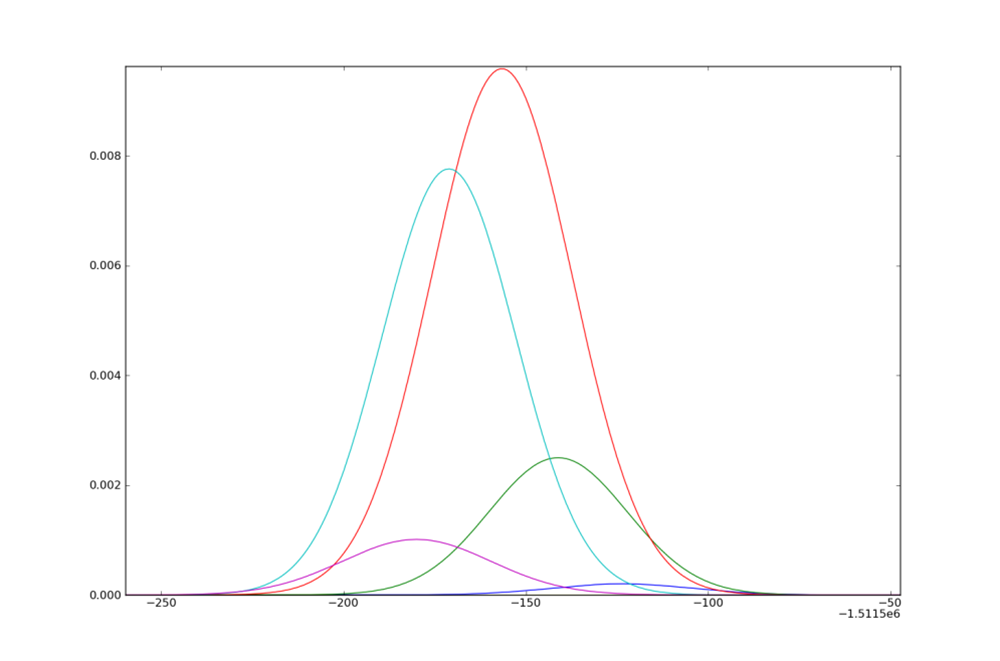
\includegraphics[width=15cm]{1st_100ns_mm_multi_gauss.png}
 \captionof{figure}{Gaussian distributions used to calculate the free energy when using the 1$^{st}$ 100ns MM energies as the substate control parameter}\label{fig:1st_100ns_mm_multi_gauss}
\end{center}


\begin{center}
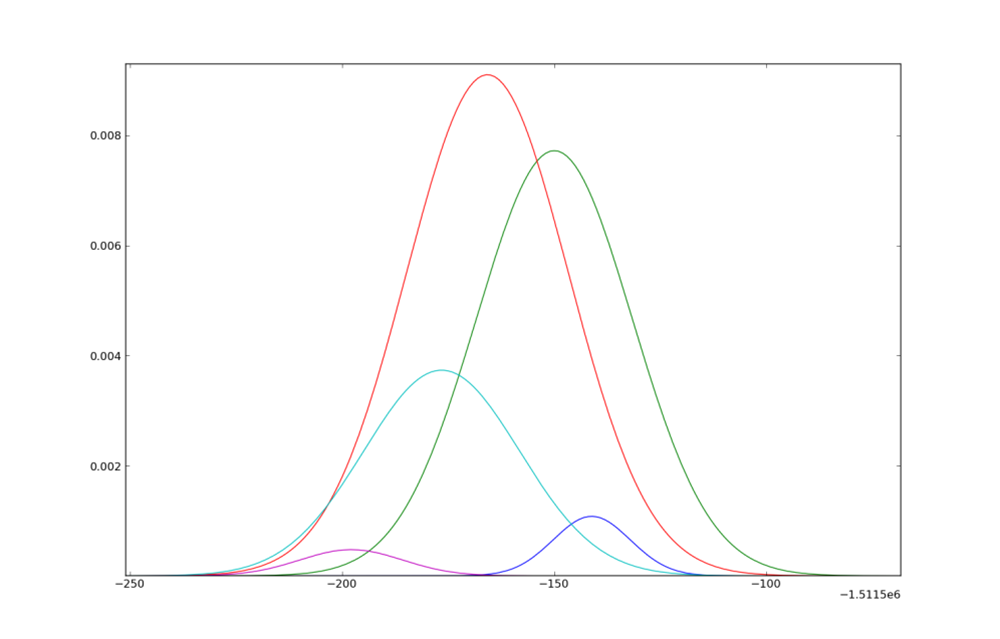
\includegraphics[width=15cm]{2nd_100ns_mm_multi_gauss.png}
 \captionof{figure}{Gaussian distributions used to calculate the free energy when using the 2$^{nd}$ 100ns MM energies as the substate control parameter}\label{fig:2nd_100ns_mm_multi_gauss}
\end{center}

The line boundaries for the MM data are shown below:

\begin{table}[ht]
  \begin{center}
  \begin{tabular}{c c c}
 & \multicolumn{2}{c}{Minimum boundary} \\
 Line colour & 1$^{st}$ 100 ns & 2$^{nd}$ 100 ns \\
 Blue & -1631.580 & -1602.100 \\
 Green & -1593.174 & -1567.220 \\
 Red & -1554.768 & -1532.340 \\
 Cyan & -1516.362 & -1497.460 \\
 Pink & -1477.956 & -1462.580 \\
 MAX VALUE & -1439.550 & -1427.700 \\
 \end{tabular}
 \end{center}
\end{table}

\begin{center}
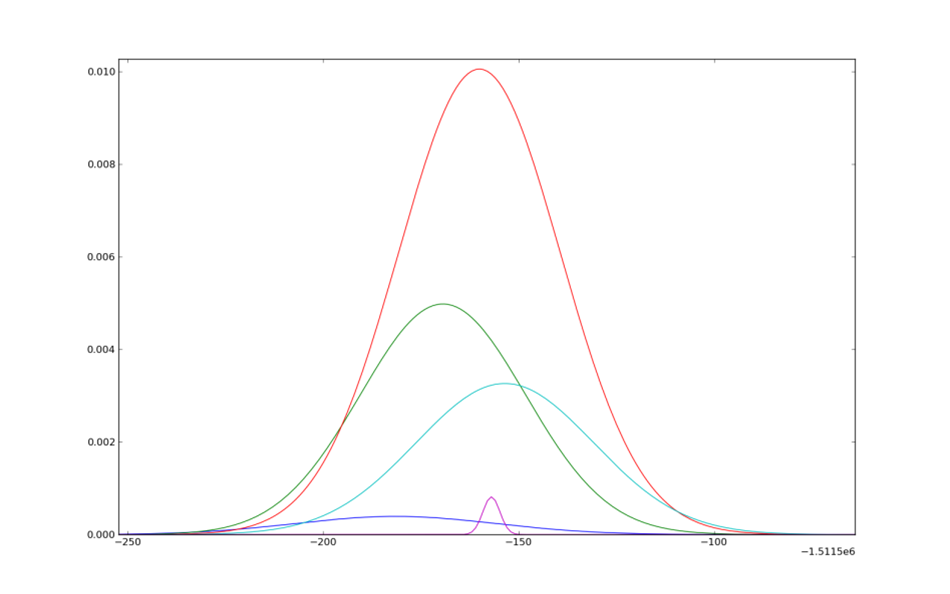
\includegraphics[width=15cm]{1st_100ns_qm_multi_gauss.png}
 \captionof{figure}{Gaussian distributions used to calculate the free energy when using the 1$^{st}$ 100ns QM energies as the substate control parameter}\label{fig:1st_100ns_qm_multi_gauss}
\end{center}

\begin{center}
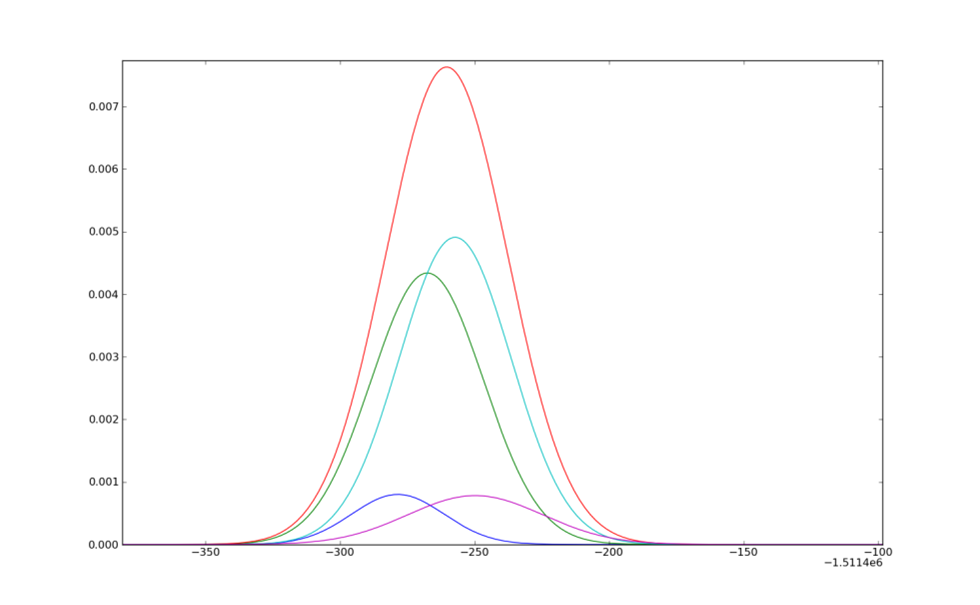
\includegraphics[width=15cm]{2nd_100ns_qm_multi_gauss.png}
 \captionof{figure}{Gaussian distributions used to calculate the free energy when using the 2$^{nd}$ 100ns QM energies as the substate control parameter}\label{fig:2nd_100ns_qm_multi_gauss}
\end{center}

The line boundaries for the QM data are shown below:

\begin{table}[ht]
  \begin{center}
  \begin{tabular}{c c c}
 & \multicolumn{2}{c}{Minimum boundary} \\
 Line colour & 1$^{st}$ 100 ns & 2$^{nd}$ 100 ns \\
 Blue & -1513266.870 & -1513255.400 \\
 Green & -1513231.992 & -1513227.316 \\
 Red & -1513197.114 & -1513199.232 \\
 Cyan & -1513162.236 & -1513171.148 \\
 Pink & -1513127.358 & -1513143.064 \\
 MAX VALUE & -1513092.480 & -1513114.980 \\
 \end{tabular}
 \end{center}
\end{table}

The free energy can then be found by applying the following equation,

\begin{equation}
\ \Delta G = -k_B T \ln \int \sum_n c_n P_n (\Delta E) \exp \left[- \frac{\Delta E}{k_BT}  \right] d \Delta E \\.
\end{equation}

The resultant free energy can be seen in table \ref{table:multi_gauss_free_energy}.

\begin{table}[ht]
 \caption{Free energies calculated by using multiple Gaussian distributions to describe the probability density}
  \begin{center}
  \begin{tabular}{c|c|c|c}
   \hline\hline
Substate parameter & 1$^{st}$ 100.0 ns & 2$^{nd}$ 100.0 ns & Difference \\
 \hline
MM energy & -1512019.13 & -1511968.77 & -50.36 \\
 \hline
QM energy & -1512221.67 & -1512171.68 & -49.99 \\
 \end{tabular}\label{table:multi_gauss_free_energy}
 \end{center}
\end{table}

Examination of the multiple Gaussian distributions used as the probability density shows in every case the center Gaussian (red) is the largest and the Gaussians used for the extremities (pink and blue) are the smallest, both of which are indications that there must be some degree of overlap for the configurational space between the MM and QM.  If there was no overlap at all, the substate Gaussians would have different proportional sizes.  This further enforces the examination of the energy distributions within the box and whisker plots previously, showing that the issue of outliers comes from rare events that are on different sides of the distributions.  Several of the substate Gaussians have low energy tails overlapping, this could have better described the low energy energy differences and perhaps have provided better convergence.  However, the produced free energies show poor convergence between simulation runs (table \ref{table:multi_gauss_free_energy}), but very good convergence between the $\Delta \Delta G$ produced by different substate diagnostic parameters.


\section{Conclusions}

The work presented within this chapter has made some progress toward calculating quantum free energies when using classical mechanics to sample structure.  Issues in convergence can be largely attributed to the inexact overlap of the configurational space.  The effect of changing this overlap was demonstrated when using charge perturbations, it is clear that even a small perturbation can cause convergence problems.  However, by using the multistate Gaussians, it has been shown that there is no bias towards either the high energy or low energy structures in the QM distributions, which proves some degree of overlap.  The box and whisker plots also defend this conclusion, with snapshots close to the median of the energy difference distribution being found on the same side of the MM and QM energy distributions.  Outlier snapshots are caused by rare events when the configurational space does not overlap, however, because of the calculation involved within the Zwanzig equation (equation \ref{eq:1_zwanzig}), these rare events dominate the free energy.

In the event of infinite sampling, this single step perturbation (SSP) method will work because all rare events will be sampled, however, this is obviously infeasible.  An alternative to this is to apply a method that will analyse whether the classically obtained structure is a good ``fit'' for a quantum ensemble.  Woods et al. \cite{mullholland_qmmm} use an acceptance criterion to converge the free energy when perturbing from MM to QM/MM.  The next chapter will apply this method, using QM/MM only as a stepping stone to the full QM.



%CLASSICAL AND QM CONFIGURATIONAL SPACE HAS SOME DEGREE OF OVERLAP

%FREE ENERGY DOMINATED BY RARE EVENTS

%BETTER SAMPLING/MORE SAMPLING NEEDED

%(EXPENSIVE)

%(MULTI TIMESTEP MONTE CARLO..)